\documentclass[sigconf]{acmart}

\usepackage{listings}
\usepackage{color}

\lstset{ % General setup for the package
basicstyle=\ttfamily\footnotesize,
    frame=tb,
    tabsize=2,
    columns=fixed,
    showstringspaces=false,
    showtabs=false,
    columns=fullflexible,
    frame=single,
    breaklines=true,
    postbreak=\mbox{\textcolor{red}{$\hookrightarrow$}\space},
    stepnumber=1,
    showstringspaces=false,
    tabsize=1,
    breakatwhitespace=false,
}


\AtBeginDocument{%
  \providecommand\BibTeX{{%
    \normalfont B\kern-0.5em{\scshape i\kern-0.25em b}\kern-0.8em\TeX}}}

\usepackage{dblfloatfix}
\usepackage[acronym]{glossaries}

\begin{document}

\newacronym{SMART}{SMART}{SeMantic AnsweR Type}
\newacronym{ATP}{ATP}{Answer Type Prediction}
\newacronym{BERT}{BERT}{Bidirectional Encoder Representations from Transformers}

\title{Semantic Answer Type Prediction 2020}

% AUTHORS:
\author{Stephan Frederik Werner Brandasu}
\affiliation{University of Stavanger}

% DATE:
\date{\today}



\begin{abstract}
We describe our solution to the \gls{SMART} prediction task 2020 for the DBpedia dataset. Our methods will take advantage of BM25 scores that get modified by the presence of specific keywords in the questions.
\end{abstract}

\keywords{information retrieval, answer category classification, answer type prediction, natural language understanding, understanding query types}

%% Remove copyright footer
\settopmatter{printacmref=false}
\setcopyright{none}
\renewcommand\footnotetextcopyrightpermission[1]{}
\pagestyle{plain}
%% ------------------------

%%
%% This command processes the author and affiliation and title
%% information and builds the first part of the formatted document.
\maketitle



\section{Introduction}
%Explain the context of the problem that you are tackling, including references to relevant literature.
\gls{ATP} is a challenging problem in the natural language processing field which is an important step to being able to understand natural language queries. Understanding the category and type of a given question is an important step in reaching this goal.

The \gls{SMART} task has provided 2 datasets, one using the DBpedia ontology and another using the Wikidata ontology.
Both datasets follow the same structure and will have a question id, a question text in natural language, an answer category and an answer type. They do differ in one sense though, If the category is a 'resource' then the types from the DBpedia dataset are different from the ones in the Wikidata dataset. This has to be taken into account when attempting to classify the questions.

The goal of this paper is to as accurately as possible classify the category and type of a natural language question from the DBpedia dataset.



\section{Related Works}

\subsection{Question word categories}
A previous submission to the \gls{SMART} task by \citet{Maryland:qwords} from the University of Maryland found that the category of an answer is highly dependent on the question words. They found for example that questions starting with 'Is' or 'Does' always expect a boolean answer and questions starting with 'when' could expect either a number or a date\cite{Maryland:qwords}. A graph showing the most common question words found by this paper can be seen in figure \ref{figure:firstquestionwords}. 

\begin{figure}[h]
    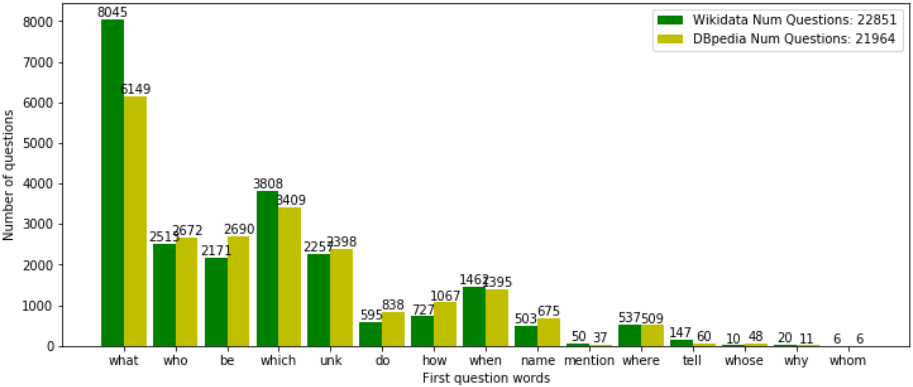
\includegraphics[width=0.48\textwidth]{figures/firstQuestionWords.png}
    \caption{"First words in sentences from Wikidata and DBpedia datasets" by \citet{Maryland:qwords}}
    \label{figure:firstquestionwords}
\end{figure}

\subsection{Most frequent resource types}
The submission by \citet{Kothen:analysis} from the University of Applied Sciences in Kothen Germany did some analysis on the dataset and found that which types of resources came up most commonly over the whole dataset. This information can be used to weigh the possible answers to try to deduce the correct answer type for a given question\cite{Kothen:analysis}. A graph showing the most common answer types found by this paper can be seen in figure \ref{figure:top10resourceanswertypes}.

\begin{figure}[h]
    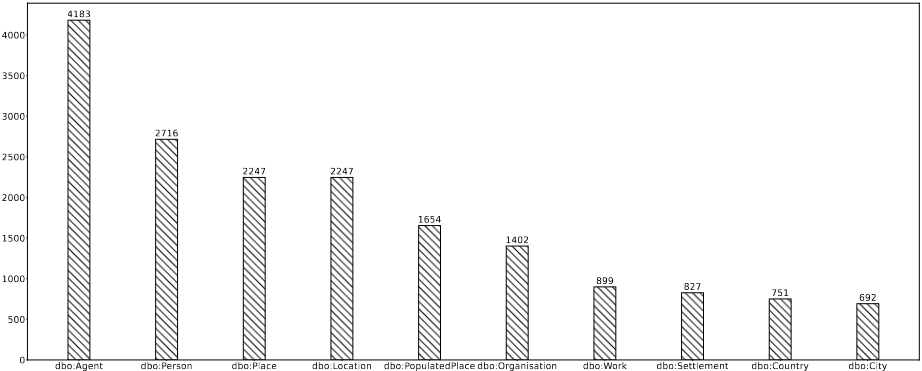
\includegraphics[width=0.48\textwidth]{figures/top10ResourceAnswerTypes.png}
    \caption{"TOP 10 resource answer types" by \citet{Kothen:analysis}}
    \label{figure:top10resourceanswertypes}
\end{figure}

\subsection{Common methods for classification}
A model used frequently used for question classification by previous submissions is \gls{BERT}\cite{maastricht:bert, heraklion:bert, tokyo:bert, uis:bert, Kothen:analysis}. 

\gls{BERT} is an open source machine learning framework used for natural language processing. The model has been pre-trained but also can be fine-tuned with your own datasets. What is unique about BERT is that it can learn bidirectional representations with transformers. This allows for much larger data sets to be analyzed more quickly since words can be processed in relation to all other words at once, instead of one at the time. Additionally by using transformers \gls{BERT} can better understand the context of a word since it compares it to all the other words at once, this makes it extremely capable for text classification tasks such as this.\cite{nvidia:bert}



\section{Problem Statement}
%Formalize the task (in terms of input and output) and specify important details about the data collection.
\subsection{Task}
The objective of this task is to take a natural language question and correctly classify the category and types expected from said question. More broadly this means that a systems needs to be created which takes a normal human written sentence and knows whether to categorise this question as a resource, a literal or as a boolean. Depending on the category it must also identify the correct types for each given category. 

A boolean can only have boolean as a type. Meanwhile a literal could be expecting a string, a date or a number as a type. Resources expect more specific type predictions. First of all they might expect more than 1 type which the other 2 categories never do. Resources could expect up to 10 types so it must be correctly deduced how many types belong to a question. These types are also expected to exist within a hierarchy based on how specific they are, the least specific should be last.

When classifying the DBpedia dataset it is important to remember that each resource type needs to be prepended with 'dbo:'.

The category and type prediction should be done in 2 steps, first handling the category of a given question and then establishing the types of that category.

\subsection{Evaluation}
To evaluate the results of the classification algorithm 2 different metrics will be used; Accuracy and $NDCG@k$. Accuracy simply tells us what percentage of the category classifications are correct. $NDCG@k$ will be computed for 2 different values of $k$; 5 and 10. This ranking will only consider literals and resources since booleans only have 1 possible type. For literals the score is either $1$ if the type is correct, or $0$ if it isn't. Resources meanwhile expect a ranked list of 10 classes so the $NDCG@K$ will score our type order based on how close it is to the ground truth order. Note that $NDCG@k$ will not penalise us for bad document outputs. 

%% finish up until here for deadline 1
\section{Baseline Method}
%Explain what you are taking as your baseline method, as well as why this is a reasonable baseline, and why you are making specific implementation choices.
\subsection{Indexing}
First we must create two different indices for each stage of question classification. The first index is a collection of both the DBpedia and the Wikidata training dataset included with the task. These datasets get combined and each question gets preprocessed. The preprocessing simply removes any punctuation and stems the questions using a Porter Stemmer. No stop word removal is done because they could be important to understanding the question. After preprocessing the questions get indexed using Elasticsearch where their document id will be the training set question id and then the document will have a field containing the question, its category and its types. 

The second index is a collection of descriptions and types belonging to descriptions from a DBpedia data dump. First we take the dump of instances from DBpedia where a page is linked to a type and we clean this list. This means that we take the page link and remove the url to only get the name. If a page has multiple types then we have to remove the number at the end of the url and merge the types together into 1 entry in the cleaned dataset.

From there we will take the dump of abstracts that link a page to a description. This description will get preprocessed like before except this time the preprocessing also removes stop words so that the descriptions should primarily contain key-words. For each description id we check if we there is a match with the same id in the instances list. If there is then we add the corresponding types to the description, if not then we don't index the description. 

\subsection{Classification}
\hfill \break
For clarity of which dataset is being talked about going forward. A question is referring to a question from the indexed training datasets. A query is referring to a question from the test dataset which is being classified. 
\hfill \break

Once these indices are in place we can start actually classifying the queries. The first step is to compare the queries to the indexed training dataset. We will use the Elasticsearch \emph{search} function which uses BM25 scoring to create a list of the most relevant questions relative to the query. We simply take the first result from \emph{search} and we use Elasticsearch \emph{get} to retrieve the category and type of the question which best matched the query.

From here we enter the second stage of classification. If the category from the first stage is either 'boolean' or 'literal' we don't do any further classification. If the category is 'resource' then we will clear the existing list of types and replace them in the following way.

In the second stage of classification we will again use Elasticsearch \emph{search} to find the best match for the query. But instead of searching the questions from the training datasets we now search the indexed collection of descriptions and types from the DBpedia data dump. The other difference for the second stage is that instead of only taking the top result, we will now try to take the top 20 results. For each result we will again use Elasticsearch \emph{get} to retrieve the types from the description. Then we will iterate through each type and add it to the list of types for the query. If the type already exists in the type list then we don't add it to avoid redundancy. We will also stop adding types once the type list has 10 entries in it due to the evaluating only considering up to 10 types. 

\subsection{Classification Reasoning}

The reason that we first compare the query to the training questions and then to the DBpedia data dump is to try to prioritise getting the "easier" categories where there are only 1 or 3 possible types correct. Doing the category prediction first using the training datasets seemed like the most intuitive way of achieving this. 

Then for the second stage, the reason we go through up to 20 results from the DBpedia data dump, even though we only want to take 10 types from the results, is that it was chosen to try to prioritise getting a better $NDCG@10$ score by trying to make sure that the classification will try to predict as many types as possible. Depending on the amount of results we won't necessarily get 10 types, but we try to get close to get as many predictions as possible.

\begin{table}[h]
    \centering
    \caption{Baseline method results}
    \begin{tabular}{c|c|c}
    $Accuracy$ & $NDCG@5$ & $NDCG@10$ \\
    \hline
    0.916 & 0.487 & 0.489
    \end{tabular}
    \label{tab:baseline_res}
\end{table}

We can see the results for the baseline methods in table \ref{tab:baseline_res}. Here we can see that the category prediction is correct a large majority of the time. The type prediction meanwhile performs worse and differently depending on how many types we consider. The results are slightly better when we look at the score for 10 types instead of 5, this makes sense considering the focus on "guessing" as many types as possible.

% finish up until here for deadline 2
\section{Advanced Method}
%Explain what you are taking as your advanced method(s), as well as why this is a promising attempt to outperform the baseline method, and why you are making specific implementation choices.
\subsection{Advanced Method 1}
For the advanced method we make some changes to the category and type prediction in an attempt to fine tune the results. First in the category prediction, before we search the indexed collection of questions, we check if the query contains the words 'how many' after each other. The chance that somebody is asking 'how many x' and isn't expecting a number as a response was decided to be basically 0. So these 2 words coming after each other will always return 'literal' as the category and 'number' as the type. 

Additionally during the category prediction we will now attempt to re-weigh the scoring by looking at the first word of the question. First the initial \emph{search} will take the top 10 results instead of only the top result. For each of these results we will save the top result from each category if it exists. From there for each top result for a given category we will increase the score based on the first word in the query.

The score increases were decided by analysing the training dataset. First finding the words that would most commonly appear at the start of sentences. Then we would check each word to see how often it appears in a given category. For example we found that when the first word is 'give' it is a resource $66\%$ of the time and a literal $33\%$ of the time. These values would be used for the score modifiers. So if a word was a resource 66\% of the time we would increase the score by $6.6$. The minimum score increase is 0.1 if it appears $1\%$ of the time and 10 if it was $100\%$ of the time.

We can see the results of these modifications in table \ref{tab:advanced1_res}.

\begin{table}[h]
    \centering
    \caption{Advanced method 1 results}
    \begin{tabular}{c|c|c}
    $Accuracy$ & $NDCG@5$ & $NDCG@10$ \\
    \hline
    0.940 & 0.499 & 0.501
    \end{tabular}
    \label{tab:advanced1_res}
\end{table}

\subsection{How the Question words were found}
To find the words that would be re-weighed we would plot the top 10 most common first words for all the categories. As an example we can see the most common first words for booleans in figure \ref{figure:top10bool}. Note that some words like 'was' has its end cut off so it comes out as 'wa'. This is due to the stemming in the preprocessing. 

\begin{figure}[h]
    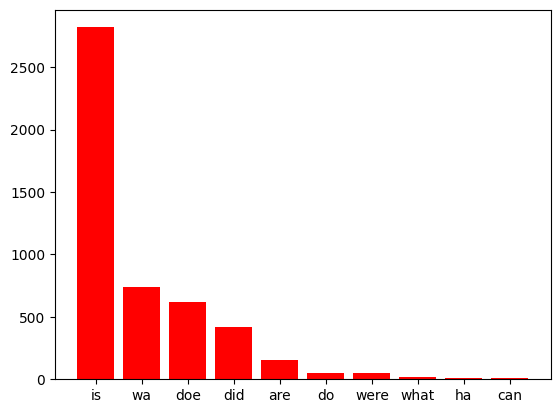
\includegraphics[width=0.48\textwidth]{figures/fwords.png}
    \caption{Top 10 most common first words for booleans}
    \label{figure:top10bool}
\end{figure}

Once we have plotted the most common words we will then check each word and get a percentage of how often it appears in every category. In listing \ref{lis:catper} we can see how this would look like. So based on this output we would give the word 'is' $9.6$ extra score if the category is a boolean. If it is a resource we will give $0.2$ extra score, and no extra score if the category is literal.

\begin{figure}[h]
    \begin{lstlisting}[caption=Checking the category percentage of words, label={lis:catper}]
        is %:  {'boolean': 0.9684065934065934, 'resource': 0.024725274725274724, 'literal': 0.006868131868131868}
        wa %:  {'boolean': 0.9547803617571059, 'resource': 0.027131782945736434, 'literal': 0.01808785529715762}
        doe %:  {'boolean': 0.9642857142857143, 'resource': 0.03260869565217391, 'literal': 0.003105590062111801}
        did %:  {'boolean': 0.9348314606741573, 'resource': 0.05393258426966292, 'literal': 0.011235955056179775}
        are %:  {'boolean': 0.968944099378882, 'resource': 0.031055900621118012}
        do %:  {'boolean': 0.8793103448275862, 'resource': 0.08620689655172414, 'literal': 0.034482758620689655}
        were %:  {'boolean': 1.0}
        what %:  {'resource': 0.7163323782234957, 'literal': 0.2823651992706434, 'boolean': 0.0013024225058609013}
        ha %:  {'boolean': 0.7857142857142857, 'resource': 0.21428571428571427}
        can %:  {'resource': 0.56, 'boolean': 0.32, 'literal': 0.12}
        \end{lstlisting}
\end{figure}



\subsection{Advanced Method 2}

The second modification made to the baseline method is in the resource type prediction. Now instead of only grabbing the resources by searching the DBpedia data dump we Additionally insert the resourced grabbed by the initial search of the training dataset. While we're adding the types from the DBpedia datadump we check if the score of the type is less than the score from the training question match. If it is then we insert the types from the training data. This way the types should be in the most relevant order. Additionally we check if the result from the type descriptions dataset is less than $\frac{1}{4}$ of the original score from the training dataset. If it is then we don't add the types since they're probably irrelevant. 

We can see the results of these modifications being combined with the modifications from advanced method 1 in table \ref{tab:advanced2_res}.

\begin{table}[h]
    \centering
    \caption{Advanced method 2 results}
    \begin{tabular}{c|c|c}
    $Accuracy$ & $NDCG@5$ & $NDCG@10$ \\
    \hline
    0.940 & 0.524 & 0.538
    \end{tabular}
    \label{tab:advanced2_res}
\end{table}


\section{Results}
%With tables and graphs, make a clear, concise, and digestible presentation of the data produced by your experiments. This includes describing the key facts and trend from your results.
The progression of the results of each method can be seen in table \ref{tab:sum_res}. Here we can see that each iteration of the advanced method improves the results of what comes before. It should be noted that 'Advanced Method 1' does not do anything to the type prediction but still sees a small improvement in the $NDCG$ scores. This is because improving the category prediction will also improve the type predictions since if we wrongly classify the category of a question by extension the types will also be wrong. 

\begin{table}[h]
\begin{center}
\caption{Summary of results}
\begin{tabular}{l|c|c|c}
     & $Accuracy$ & $NDCG@5$ & $NDCG@10$ \\
    \hline
    Baseline & 0.916 &  0.487 & 0.489 \\
    Advanced Method 1 & 0.940 & 0.499 &  0.501 \\
    \textbf{Advanced Method 2} & \textbf{0.940} & \textbf{0.524} &  \textbf{0.538} \\
\end{tabular}
\label{tab:sum_res}
\end{center}
\end{table}

Overall while the score weighing works, it only improves the results in small effect. What ended up being a lot more meaningful was also adding the types from the training questions to resource type answers instead of only using the types from the DBpedia dump.


\section{Discussion and Conclusions}
%Summarize and discuss different challenges you faced and how you solved those. Include interpretations of the key facts and trends you observed and pointed out in the Results section. Which method performed best, and why? Speculate: What could you have done differently, and what consequences would that have had?
\subsection{Algorithm Discussion}
Advanced method 1 Ended up being surprisingly effective at improving the category classification considering how simple the logic of what it actually does is. Given more time it would have been possible to experiment with higher score multipliers for certain words, or maybe giving negative score multipliers. But this would maybe go too much against what the initial scoring does, negatively affecting the result. 

Advanced method 2 does a good job at improving the type accuracy for resources but it's still missing a system to handle the type hierarchy so the types get all mixed up. Additionally the limitation built in to try to avoid less relevant types being added doesn't seem to do much. 

\subsection{Indexing Challenges}
The main challenge during the project was correctly and effectively indexing the DBpedia instance types and abstracts. These datasets are huge so they almost required to use an industrial strength solution like Elasticsearch to get any sort of acceptable performance out of the program using Python. I tried to only index descriptions from the abstracts file that would have matching types, but this ended up with a very large amount of descriptions not being included which is a bit suspicious. It is possible that something went wrong with the url stripping for the id of each description and the types, so they weren't matching correctly. But I double checked the id's in both datasets after cleaning and it looked normal. 

%%
%% If your work has an appendix, this is the place to put it.
%\appendix

%\section{Appendix}


%%
%% The next two lines define the bibliography style to be used, and
%% the bibliography file.
\bibliographystyle{ACM-Reference-Format}
\bibliography{base}

\newpage
\appendix
\section{GitHub}
The project code and datasets can be found here:

\href{https://github.com/sbthepotato/DAT640-Project-22H}{github.com/sbthepotato/DAT640-Project-22H}

\section{Division of Work During the Project}

The whole project was completed by me so this is not relevant.


\end{document}
\endinput
